\documentclass{report}

\input{preamble}
\input{macros}
\input{letterfonts}

\title{\Huge{Math 244}}
\author{\huge{PSET 3}}
\date{Feb 10 2025}

\begin{document}

% Define some pastel colors
\definecolor{pastelPink}{HTML}{ffb3ba}     % "#ffb3ba"
\definecolor{pastelBlue}{HTML}{b3cde0}     % "#b3cde0"
\definecolor{pastelGreen}{HTML}{ccebc5}    % "#ccebc5"
\definecolor{pastelLavender}{HTML}{c6aed8} % "#c6aed8"

\maketitle
\newpage% or \cleardoublepage
% \pdfbookmark[<level>]{<title>}{<dest>}
\pdfbookmark[section]{\contentsname}{toc}
\tableofcontents
\pagebreak

\section*{2.3 Prob 1}
\addcontentsline{toc}{section}{Prob 1}

\qs{}{
  How many linear extensions of $\mathcal{B}_2$ are there, and what about $\mathcal{B}_3$?
}



\begin{center}
  \begin{tikzpicture}[scale=1.0, 
      every node/.style={circle, draw, thick, minimum size=10mm, inner sep=0pt, font=\footnotesize}]
      
    % First lattice: B2 on the left
    \node (topB2) at (-4,1.5) [fill=pastelPink] {\(\{a,b\}\)};
    \node (aB2)   at (-5,0)   [fill=pastelBlue] {\(\{a\}\)};
    \node (bB2)   at (-3,0)   [fill=pastelBlue] {\(\{b\}\)};
    \node (botB2) at (-4,-1.5) [fill=pastelLavender] {\(\varnothing\)};

    % -- B2 edges --
    \draw[thick] (topB2) -- (aB2);
    \draw[thick] (topB2) -- (bB2);
    \draw[thick] (aB2) -- (botB2);
    \draw[thick] (bB2) -- (botB2);

    % Label for B2
    \node[draw=none, fill=none, below=8mm] at (-4,-2.2) {\(\mathbf{B_2}\)};

    % Second lattice: B3 on the right
    \node (top) at (2,3) [fill=pastelPink]   {\(\{a,b,c\}\)};
    \node (ab)  at (0,1.5) [fill=pastelBlue]    {\(\{a,b\}\)};
    \node (ac)  at (2,1.5) [fill=pastelBlue]    {\(\{a,c\}\)};
    \node (bc)  at (4,1.5) [fill=pastelBlue]    {\(\{b,c\}\)};
    \node (a)   at (0,0) [fill=pastelGreen]   {\(\{a\}\)};
    \node (b)   at (2,0) [fill=pastelGreen]   {\(\{b\}\)};
    \node (c)   at (4,0) [fill=pastelGreen]   {\(\{c\}\)};
    \node (bot) at (2,-1.5) [fill=pastelLavender] {\(\varnothing\)};

    % -- B3 edges --
    \draw[thick] (top) -- (ab);
    \draw[thick] (top) -- (ac);
    \draw[thick] (top) -- (bc);

    \draw[thick] (ab) -- (a);
    \draw[thick] (ab) -- (b);
    \draw[thick] (ac) -- (a);
    \draw[thick] (ac) -- (c);
    \draw[thick] (bc) -- (b);
    \draw[thick] (bc) -- (c);

    \draw[thick] (a) -- (bot);
    \draw[thick] (b) -- (bot);
    \draw[thick] (c) -- (bot);

    % Label for B3
    \node[draw=none, fill=none, below=8mm] at (2,-2.2) {\(\mathbf{B_3}\)};
  \end{tikzpicture}
\end{center}


\begin{RemarkWithLily}{For Prob 1}
  FFor $\mathcal{B}_2$ there are two linear extensions because the linear extension must respect and preserve the original partial order 
  so the empty set must be first and the set $\{a,b\}$ must be at the top which means ther variation in ordering the remaining elements is $2!$ as those are the elements below 
  $\{a,b\}$ and above the empty set. 

  \medskip

  For $\mathcal{B}_{3}$ there are 36 possible linear extensions. Since the linear extension needs to preserve teh original 
  partial order than that means the unique top element and unique bottom element of the set $\{a,b,c\}$ and the empty set must be the last and first 
  element of any linear extension respectively. For the remaining elements the sets with cardinlaties 1 must all come before the sets of cardinality 2 
  but there are $3$ sets of cardinality 1 that can be ordered in $3!$ ways as there are 3 options for the first one, 2 for the second, and 1 for the last one. 
  This logic also applies to the 3 sets of cardinality of 2 that must all go after the sets of cardinality 1 and before the unique top element of 
  cardinality 3 so there are $3!$ ways to order those. This makes the total possible linear extensions the result of 
  multiplying the possibilities of each possible way of ordering the elements so $1 \cdot 3! \cdot 3! \cdot 1$ which is $36$. 
\end{RemarkWithLily}




\section*{Bonus Problem}
\addcontentsline{toc}{section}{Bonus Prob}

\qs{}{
  Prove that not every
  finite poset admits an embedding into the poset $( \mathbb{N}^2, \preceq)$, where
  $(x_1, y_1)\preceq (x_2, y_2)$ if and only if $x_1 \leq x_2$ and $y_1 \leq y_2$.
}

\section*{2.4 Prob 3}
\addcontentsline{toc}{section}{Prob 2}

\qs{}{
  Find a sequence of real numbers of length 16 that contains no monotone
  subsequence of length 5.
}

\begin{center}
  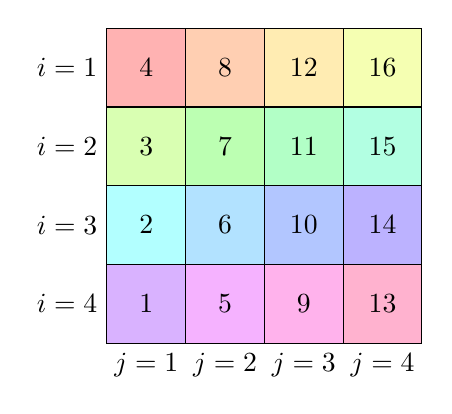
\begin{tikzpicture}[scale=1]
    % Loop over rows i=1..4 and columns j=1..4
    \foreach \i in {1,2,3,4} {%
      \foreach \j in {1,2,3,4} {%
        % Compute the value to display
        \pgfmathtruncatemacro{\val}{4*(\j-1) + (5-\i)}
        % Compute a hue between 0 and 1 depending on row and column.
        \pgfmathsetmacro{\hue}{((\i-1)*4 + (\j-1))/16}
        %
        % --- Convert HSV (hue, 0.3, 1) to RGB ---
        % Compute H' = 6 * hue.
        \pgfmathsetmacro{\Hprime}{6*\hue}
        % Determine the sector (an integer between 0 and 5)
        \pgfmathtruncatemacro{\sector}{floor(\Hprime)}
        % The fractional part
        \pgfmathsetmacro{\f}{\Hprime - \sector}
        % p is constant because saturation is 0.3:
        \pgfmathsetmacro{\pval}{0.7} % since 1 - 0.3 = 0.7
        % q and t depend on f:
        \pgfmathsetmacro{\qval}{1 - \f*0.3}
        \pgfmathsetmacro{\tval}{1 - (1-\f)*0.3}
        %
        % Now set r,g,b based on the sector.
        % We use TeX conditionals (\ifcase ... \fi). The numbers will be stored in
        % macros \rval, \gval, \bval.
        \ifcase\sector
          \def\rval{1}%
          \def\gval{\tval}%
          \def\bval{\pval}%
        \or
          \def\rval{\qval}%
          \def\gval{1}%
          \def\bval{\pval}%
        \or
          \def\rval{\pval}%
          \def\gval{1}%
          \def\bval{\tval}%
        \or
          \def\rval{\pval}%
          \def\gval{\qval}%
          \def\bval{1}%
        \or
          \def\rval{\tval}%
          \def\gval{\pval}%
          \def\bval{1}%
        \or
          \def\rval{1}%
          \def\gval{\pval}%
          \def\bval{\qval}%
        \fi
        %
        % Draw the cell using the computed RGB color.
        % The fill syntax here uses the "rgb" model.
        \node[draw,
              fill={rgb,1:red,\rval; green,\gval; blue,\bval},
              minimum width=1cm,
              minimum height=1cm]
              at (\j,-\i) {\(\val\)};
      }%
    }
    
    % Place row labels to the left (using anchor=east so they don’t touch the boxes)
    \node[anchor=east] at (0.5, -1) {\(i=1\)};
    \node[anchor=east] at (0.5, -2) {\(i=2\)};
    \node[anchor=east] at (0.5, -3) {\(i=3\)};
    \node[anchor=east] at (0.5, -4) {\(i=4\)};
    
    % Place column labels below (using anchor=north)
    \node[anchor=north] at (1, -4.5) {\(j=1\)};
    \node[anchor=north] at (2, -4.5) {\(j=2\)};
    \node[anchor=north] at (3, -4.5) {\(j=3\)};
    \node[anchor=north] at (4, -4.5) {\(j=4\)};
  \end{tikzpicture}
\end{center}

\bigskip

\noindent
Reading the cells row by row (from top row to bottom row) gives the sequence:
\[
4, 8, 12, 16,\quad
3, 7, 11, 15,\quad
2, 6, 10, 14,\quad
1, 5, 9, 13.
\]

\exrose{For Prob 2}{
  AArray: [1,2,3,4,5,6,7,8,9,10,11,12,13,14,15,16] 
}


\section*{2.4 Prob 4}
\addcontentsline{toc}{section}{Prob 3}

\qs{}{
  Prove the following strengthening of Theorem 2.4.6: Let $k, \ell$ be
  natural numbers. Then every sequence of real numbers of length $k \ell + 1$
  contains a nondecreasing subsequence of length $k+1$ or a decreasing subsequence of
  length $ \ell +1$.
}


\begin{proofWithHibiscus}
  Let a sequence $(x_1, x_2, \ldots, x_{kl+1})$ be a sequence of real numbers and let $X = \{1,2, \ldots , kl + 1 \}$. \\
  Define a relation $\preceq$ on $X$ by 
  \[ i \leq j \quad iff \quad i \leq j \text{ and } x_{i} \leq x_{j} \]
  \begin{ClaimWithMagnolia}
    $\preceq$ is an ordering
    \medskip

    reflexive: $i \leq i$ for all $i$ since $i \leq i$ and $x_{i} \leq x_{i}$ 

    \medskip

    antisymetric: Suppose $i \leq j$ and $j \leq i$. Then $i \leq j$ and $j \leq i$ and $x_i \leq x_j$ and $x_j \leq x_i$. \\
    implies $i = j$ and $x_i = x_j$ 

    \medskip

    transitive: suppose $i \leq j$ and $j \leq k$. Want to show $i \leq k$. \\
    $i \leq j$ implies $i \leq j$ and $x_i \leq x_j$. \\
    $j \leq k $ implies $j \leq k$ and $x_j \leq x_k$. But then $i \leq k$ and $x_i \leq x_k$.\\ 
    which implies $ i \preceq k$ 
  \end{ClaimWithMagnolia} 

  by the theorem that for every finite ordered set $ P = (Xm \preceq)$ we have 
  \[ \alpha (P) \cdot \omega (P) \geq |X| \] 
  we then have 
  \[ \alpha (P) \cdot \omega (P) \geq |kl + 1|\]
  
  \medskip 
  So either 
  \begin{enumerate}
    \item $\alpha (X, \preceq) > l + 1 $
    \item $\omega (X, \preceq) > k + 1 $
  \end{enumerate}

  If $1$, then $(X, \preceq )$ has an independent set of size $l +1$ \\ 
  We then have 
  \[i_1 < i_2, \ldots , i_l+1\]
  \[ x_{i{1}} \geq x_{i_{2}}, \geq , x_{i_{k+1}}\] 

  \smallskip


  If $2$, then $(X, \preceq )$ has a chain for length $k + 1$ 
  We then have 
  \[ i_1 < i_2, \ldots , i_k+1 \] 
  \[ x_{i{1}} \leq x_{i_{2}}, \ldots , x_{i_{k+1}}\] 



\end{proofWithHibiscus}

\section*{3.1 Prob 2}
\addcontentsline{toc}{section}{Prob 4}

\qs{}{
  Determine the number of ordered pairs $(A, B)$, where $A \subseteq B \subseteq \{ 1, 2, \ldots, n \}$.
}

\section*{3.1 Prob 6}
\addcontentsline{toc}{section}{Prob 5}

\qs{}{
  Show that a natural number $n \ge 1$ has an odd number of divisors
  (including 1 and itself) if and only if $\sqrt{n}$ is an integer. {\it The textbook
  has a hint to this problem in the back.}
}

\end{document}